\section{Introduzione}

\subsection{Obiettivo}

Vogliamo misurare il tasso per unità di superficie orizzontale
dei raggi cosmici che passano nel laboratorio.
Vedremo che possiamo misurare solo il tasso di muoni.

\subsection{Apparato}
% ho aggiunto la h perché non si può iniziare un testo con una figura ed è quello che è successo dopo aver aggiunto \newpage
\begin{figure}[h]
	\center
	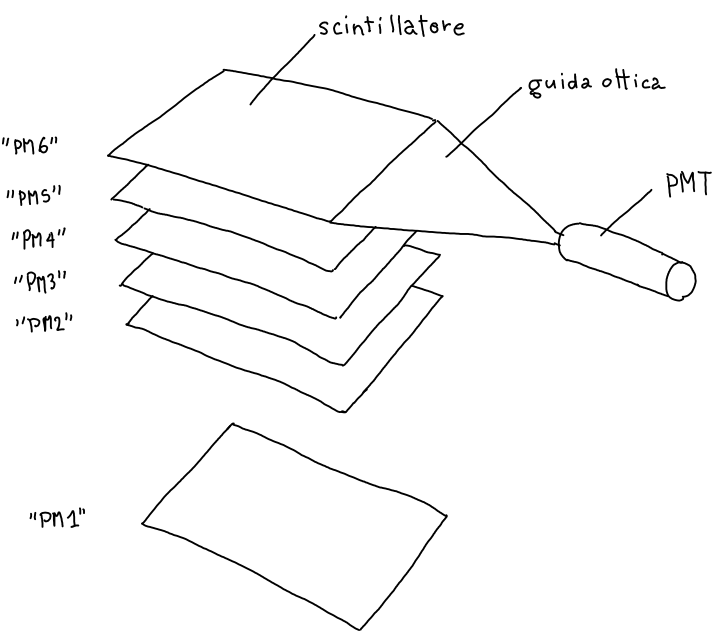
\includegraphics[width=\textwidth]{apparato}
	\caption{\label{fig:apparato}
	Apparato di misura.
	La struttura portante non è disegnata.
	La guida ottica e il tubo fotomoltiplicatore (PMT) sono disegnati solo per il PM6.}
\end{figure}

Abbiamo a disposizione 6 lastre di scintillatore plastico
posizionate orizzontali e allineate verticalmente,
che non possiamo spostare,
collegate a tubi fotomoltiplicatori (vedi \autoref{fig:apparato}).
\marginpar{Aggiungere miniscint.}
